%
% abstieg.tex
%
% (c) 2024 Prof Dr Andreas Müller
%
\begin{figure}
\centering
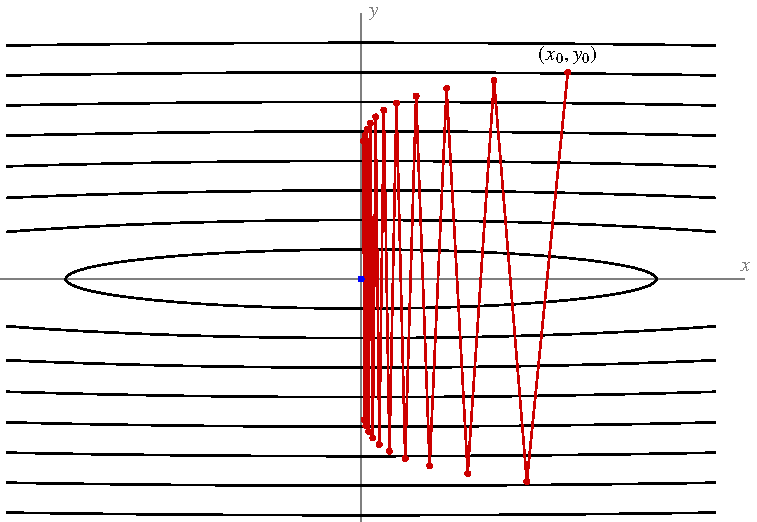
\includegraphics{chapters/070-direkt/images/abstieg.pdf}
\caption{Gradientabstieg für die Funktion $f(x,y)=x^2+100y^2$.
Weil die Ableitung entlang der $x$-Achse sehr viel kleiner ist als
die Ableitung entlang der $y$-Achse, ist der Abstieg mit 
$(x_{k+1},y_{k+1}) = (x_k,y_k) -\alpha \operatorname{grad}f(x_k,y_k)$
mit dieser Wahl von $\alpha$ sehr langsam.
Die Konvergenz hängt kritisch von der geeigneten Wahl von $\alpha$ ab.
\label{buch:direkt:gradient:fig:abstieg}}
\end{figure}
